%%%%%%%%%%%%%%%%%%%%%%% file template.tex %%%%%%%%%%%%%%%%%%%%%%%%%
%
% This is a general template file for the LaTeX package SVJour3
% for Springer journals.          Springer Heidelberg 2010/09/16
%
% Copy it to a new file with a new name and use it as the basis
% for your article. Delete % signs as needed.
%
% This template includes a few options for different layouts and
% content for various journals. Please consult a previous issue of
% your journal as needed.
%
%%%%%%%%%%%%%%%%%%%%%%%%%%%%%%%%%%%%%%%%%%%%%%%%%%%%%%%%%%%%%%%%%%%
%
% First comes an example EPS file -- just ignore it and
% proceed on the \documentclass line
% your LaTeX will extract the file if required
\begin{filecontents*}{example.eps}
%!PS-Adobe-3.0 EPSF-3.0
%%BoundingBox: 19 19 221 221
%%CreationDate: Mon Sep 29 1997
%%Creator: programmed by hand (JK)
%%EndComments
gsave
newpath
	20 20 moveto
	20 220 lineto
	220 220 lineto
	220 20 lineto
closepath
2 setlinewidth
gsave
	.4 setgray fill
grestore
stroke
grestore
\end{filecontents*}
%
\RequirePackage{fix-cm}
%
%\documentclass{svjour3}                     % onecolumn (standard format)
\documentclass[smallcondensed]{svjour3}     % onecolumn (ditto)
%\documentclass[smallextended]{svjour3}       % onecolumn (second format)
%\documentclass[twocolumn]{svjour3}          % twocolumn
%
\smartqed  % flush right qed marks, e.g. at end of proof
%
\usepackage{algorithmic}
\usepackage{amsmath,amssymb,amsfonts}
\usepackage{enumerate}
\usepackage{wrapfig}
\usepackage{graphicx}
\usepackage{appendix}
\usepackage{graphicx}
\usepackage{amsmath}
\usepackage{caption}
\usepackage{subfigure}
\usepackage{makecell}
\usepackage{multirow}
\usepackage{booktabs}
\usepackage{threeparttable}
\usepackage{geometry}
\usepackage{float}
\usepackage{indentfirst}
\usepackage[colorlinks,
linkcolor=blue,
anchorcolor=black,
citecolor=blue]{hyperref}
\geometry{top=2.5cm,bottom=2.5cm}
%
% \usepackage{mathptmx}      % use Times fonts if available on your TeX system
%
% insert here the call for the packages your document requires
%\usepackage{latexsym}
% etc.
%
% please place your own definitions here and don't use \def but
% \newcommand{}{}
%
% Insert the name of "your journal" with
% \journalname{myjournal}
%
\begin{document}
	
\title{Key Information Matching in Vision-and-language Navigation%\thanks{Grants or other notes
		%about the article that should go on the front page should be
		%placed here. General acknowledgments should be placed at the end of the article.}
}
	%\subtitle{Do you have a subtitle?\\ If so, write it here}
	
	%\titlerunning{Short form of title}        % if too long for running head
	
	\author{xx* $^{1}$ \and xx $^{1}$ \and xx*$^{1}$ \and  xx $^{1}$ \and  xx $^{1}$ \and xx $^{1}$ \and xx $^{1}$}
	
	%\authorrunning{Short form of author list} % if too long for running head
	
	\institute{xx* \at
		\email{xx}   
		\\
		\and
		xx \at
		\email{xx \\} 
		\and
		xx* \at
		\email{xx \\} 
		%             \emph{Present address:} of F. Author  %  if needed
		\\
		$^{1}$  Faculty of Robot Science and Engineering, Northeastern University, Shenyang 110819, China 
	}
	
	\date{Received: date / Accepted: date}
	% The correct dates will be entered by the editor
	
	
\maketitle
\begin{abstract}
		
With the rapid growth of computer vision and natural language processing technologies, more and more researchers have paid attention on the visual and language navigation which is one of the most important tasks in multimodal intelligence. In order to optimize the effect of this task, how to meticulously integrate the multi-modal information is crucial. However, the existing model is only achieved through simple data enhancement or expansion, which is obviously far from extracting the internal connections between different modalities. In this paper, we propose a new multimodal matching method and a more flexible navigation self-correction module to overcome these challenges, which is a brand new neural network model called Key Information Matching Network (KIM-Net). Our KIM-Net consists of two matching modules, the visual matching module(V-mat) and the trajectory matching module(T-mat). Specifically, V-mat is to match the target information extracted from the vision with the entity information extracted from the instruction. T-mat is to match trajectory features to instructions. In the original visual and linguistic information, benefiting from the collaborative learning of the V-mat and the T-mat, our KIM-Net has the ability to abstract the key points between different modalities. The performance of the proposed model on various operations is then experimentally demonstrated and compared with other models using the Matterport3D Simulator and room-to-room (R2R) benchmark dataset. 
		\keywords{Vision-and-language Navigation \and Cross-modal Matching \and Self-correction Module  \and Key Information Matching Network}
		% \PACS{PACS code1 \and PACS code2 \and more}
		% \subclass{MSC code1 \and MSC code2 \and more}
		
\end{abstract}
	
\section{Introduction}
\label{intro}
	
The VLN task (Visual and Language Navigation) is to allow the agent to follow the natural language instructions to navigate. This task needs to understand the natural language instructions and the image information that can be seen in the perspective at the same time, and then make the status in the environment. The corresponding action finally reaches the target position. In recent years, Anderson \cite{anderson2018vision} first proposed a relatively simple sequence (Seq2Seq) type neural network model in which an action sequence is output from two input sequences. Then various data augmentation techniques were used to solve the problem of insufficient R2R data set for training the model, including Fried \cite{fried2018speaker}, Zhu \cite{zhu20201vision}, Jain \cite{jain2019stay}. Therefore, promoting the solution of this problem and focusing on improving the ability of perceptual visual and language input cross-modal matching has become the focus of research in this field.

Improving the ability to perceive the cross-modal matching of visual and language input is also very helpful for perfecting multimodal intelligence tasks in other fields. For example, visual question answering (VQA) \cite{antol2015vqa}, which generates answers to natural language questions on the presented images; image/video subtitle generation, generates description text on the premise of understanding the input image or video content \cite{das2017visual}, etc. If there is no way to improve the quality of the input, and just import it into the overall network without processing, a lot of useful information will be lost. Therefore, improving the cross-modal matching ability of perceptual vision and language input is of great significance to the optimization of the entire multimodal intelligence task.

It is challenging to improve the cross-modal matching ability of perceptual visual and language input for two reasons \cite{fried2018speaker,landi2019embodied,hwang2021joint}. First of all, we cannot accurately predict the key features of visual and textual information, including landmark objects in the scene or landmark direction words under instructions. Secondly, for complex indoor scenes, the inner connection between perceived visual and language input may only be reflected in some key information. If detailed analysis is not targeted, this will increase the challenge of the task.
	
In order to overcome these challenges, we propose a new multimodal matching method and navigation self-correction module. The multimodal matching method is a new neural network model KIM-Net (Key Information Matching Network). The main idea is to match the image information obtained by the visual with the entity extracted from the language input. In the original visual and linguistic information, it focuses on the matching of entity information in the data stream, thereby improving the overall cross-modal matching ability. In view of the fact that the traditional processing method only improves the matching effect by increasing the number, it greatly ignores the characteristics of the data set itself. Therefore, we follow the example of ordinary people in the process of path finding, which will give priority to matching whether to arrive at a key location, so as to determine whether to complete the navigation at this stage and proceed to the next stage of trajectory planning. Not only that, we also sample the path generated by the action predictor as the third type of data information to match the text instructions. In addition, the heuristic self-correction module is applied to the path after the matching score is lower than the threshold, it can be self-corrected to the previous stage, and the gated attention module is used to retrain and adjust the parameters to plan a more reliable path. Thereby improving the accuracy of reaching the designated destination. In general, our contributions include:

\begin{itemize}
		\item[](1) A new neural network model KIM-Net is developed, which uses the information after image target recognition to match the extracted features of language entities to optimize the utilization of dataset.
		\item[](2) The Self-calibration module based on heuristics makes the generated path match the text instruction, and retrains the parameters at the appropriate position to achieve the effect of optimizing the path and improving the robustness of the entire network.
		\item[](3) We have compared the result with baseline on the R2R dataset, and the experimental results show that the KIM-Net network can greatly improve the navigation accuracy of VLN tasks.
\end{itemize}
\section{Motivation}
	
In this section, we first explain that it is universal for the alignment of visual features and language features to be ignored. Then, introduce our preliminary idea. Finally, in response to the above ideas, the measures to be taken are proposed.
\vspace{-1em}
\subsection{Current Situation}	

\begin{figure*}[h]

	\centering
	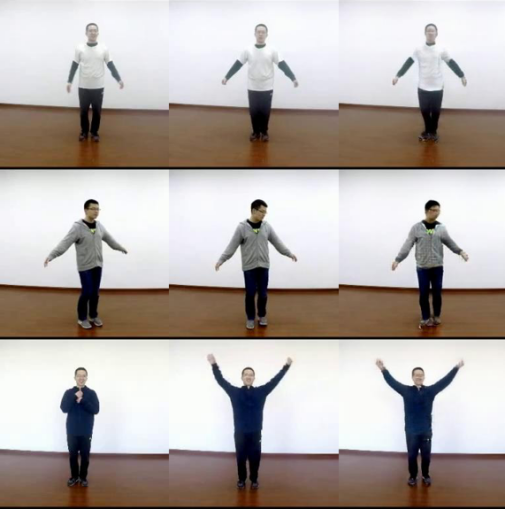
\includegraphics[scale=1]{image01.png}
	\caption{Examples of vision and language navigation (VLN) tasks.}
	\label{image01}
\end{figure*}

As Figure \ref{image01} shows, the perceptual visual information of the VLN task contains a large amount of environmental information \cite{huang2019transferable}, such as various tables, chairs, decorations, etc. in the vision. Natural language instructions include requiring the agent to perform high-level actions \cite{majumdar2020improving}, such as "walk to the lamp and stop" and Various advanced operations including "turning before the green plants". Therefore, the VLN agent is very important for the detailed processing of the two types of information. It needs to acquire knowledge of its location in the current environment to determine the next action; it needs to identify the landmark in the input image mentioned in the instruction; and it needs to choose the low-level action to implements the high-level action in accordance with the instruction.

In particular, the agent should be able to perform alignment and grounding of multimodal input data to understand the natural language instructions coherently in relation to the real-time input images \cite{qi2020object}. However, the previous work mainly focused on increasing the amount of input data, ignoring the matching between the target information and the key information of the text command under the panoramic vision. This leads to the fact that when the two features are matched, some useless features are taken into account too much, so that when input to the action prediction module, actions that cannot match the instructions are generated \cite{ma2019regretful}. After serialization, the generated trajectory is even more deviated from the original predetermined route, resulting in the poor navigation accuracy.
\vspace{-1em}
\subsection{Our Discovering}	

In response to the above-mentioned situation, we found that in the data set, the detailed matching information between perceptual vision and text instructions is often ignored. This phenomenon is not only in the R2R dataset, but also in other related fields, such as dialogue navigation, outdoor scene navigation, etc \cite{nguyen2019help,yan2019cross,chen2019touchdown}. However, this information can be extracted and reasonably used. As shown in Figure \ref{image02}, we extracted the keywords kitchen, hallway, sitting area, couch of the text instruction and the target features of the visual information have a certain corresponding relationship. The rest of the conjunctions, etc., have no corresponding goals in the visual information, and the most important keywords occupy a relatively small proportion in the entire text, which will not play a leading role in the entire model \cite{hao2020towards}. If in the model training process, we can train the dominant module as an auxiliary feature of the model, which will help improve the navigation accuracy of the entire VLN task.

\begin{figure*}[h]
	\centering
	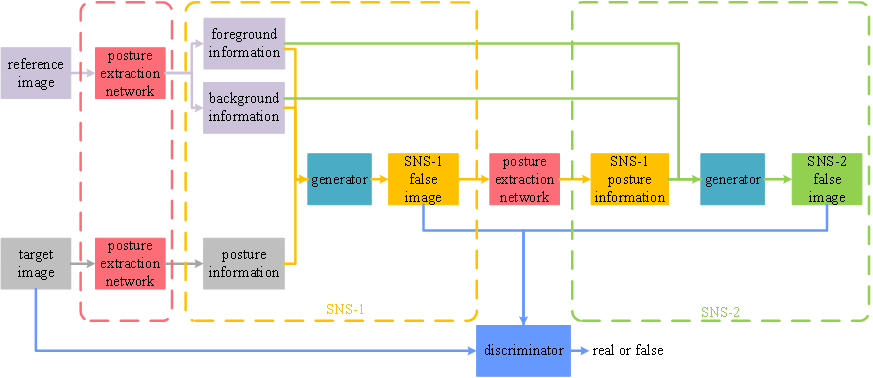
\includegraphics[scale=1]{image02.png}
	\caption{Examples of the keywords kitchen, hallway, sitting area, couch of the text instruction and the target features of the visual information have a certain corresponding relationship.}
	\label{image02}
	\vspace{-2em}
\end{figure*}

\subsection{Our Method Brief Introduction}

Based on the above description, we found that alignment matching based on the target features of the perceptual vision and the keywords of the text instruction can improve the cross-modal matching ability, and can optimize the limitation of simply expanding the amount of data to improve the network effect. This method makes full use of the subtle connections between the two modalities, matches directly from the details, grasps the impact of key information in the entire scene, and greatly optimizes the data input quality of the entire network. Based on this phenomenon, we propose the KIM-Net network, a cross-modal data fusion model based on key information matching, to solve the problem that the existing methods cannot make full use of the internal characteristics of the dataset.

\section{Model Design}
	
Based on the above motivation, we propose the KIM-Net model, that matches the information after image target recognition with the features extracted from language entities. In this section, we will introduce the details of the KIM-Net network. The KIM-Net contains two modules: visual instruction matching module and trajectory instruction matching module. as the Figure \ref{image03} shows. In the visual instruction matching module, we use the Yolo algorithm to extract the object features after target recognition and the word features processed by the entity extraction component of the instruction, compare them and input them into the action prediction module to guide the generation of navigation actions \cite{redmon2016you}.
\vspace{-2em}
\begin{figure*}[h]
	\centering
	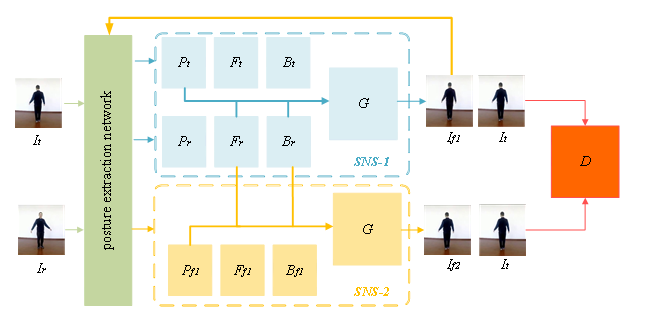
\includegraphics[scale=1]{image03.png}
	\caption{Schema of the proposed architecture for VLN. The input instruction is vision, instruction and trajectory. The KIM-Net consists of Key information match module, Cross-model guide module and Self-calibration module.}
	\label{image03}
\end{figure*}

In order to further improve the overall integrity of the navigation, we introduced a self-correcting trajectory module that matches the path and the instruction. In this module, we refer to the feedback ideas of Ke \cite{ke2019tactical}, improve the relevant evaluation score indicators, and increase the robustness of the entire system.

\subsection{Review of Target Detection Component}

\begin{figure*}[h]
	\centering
	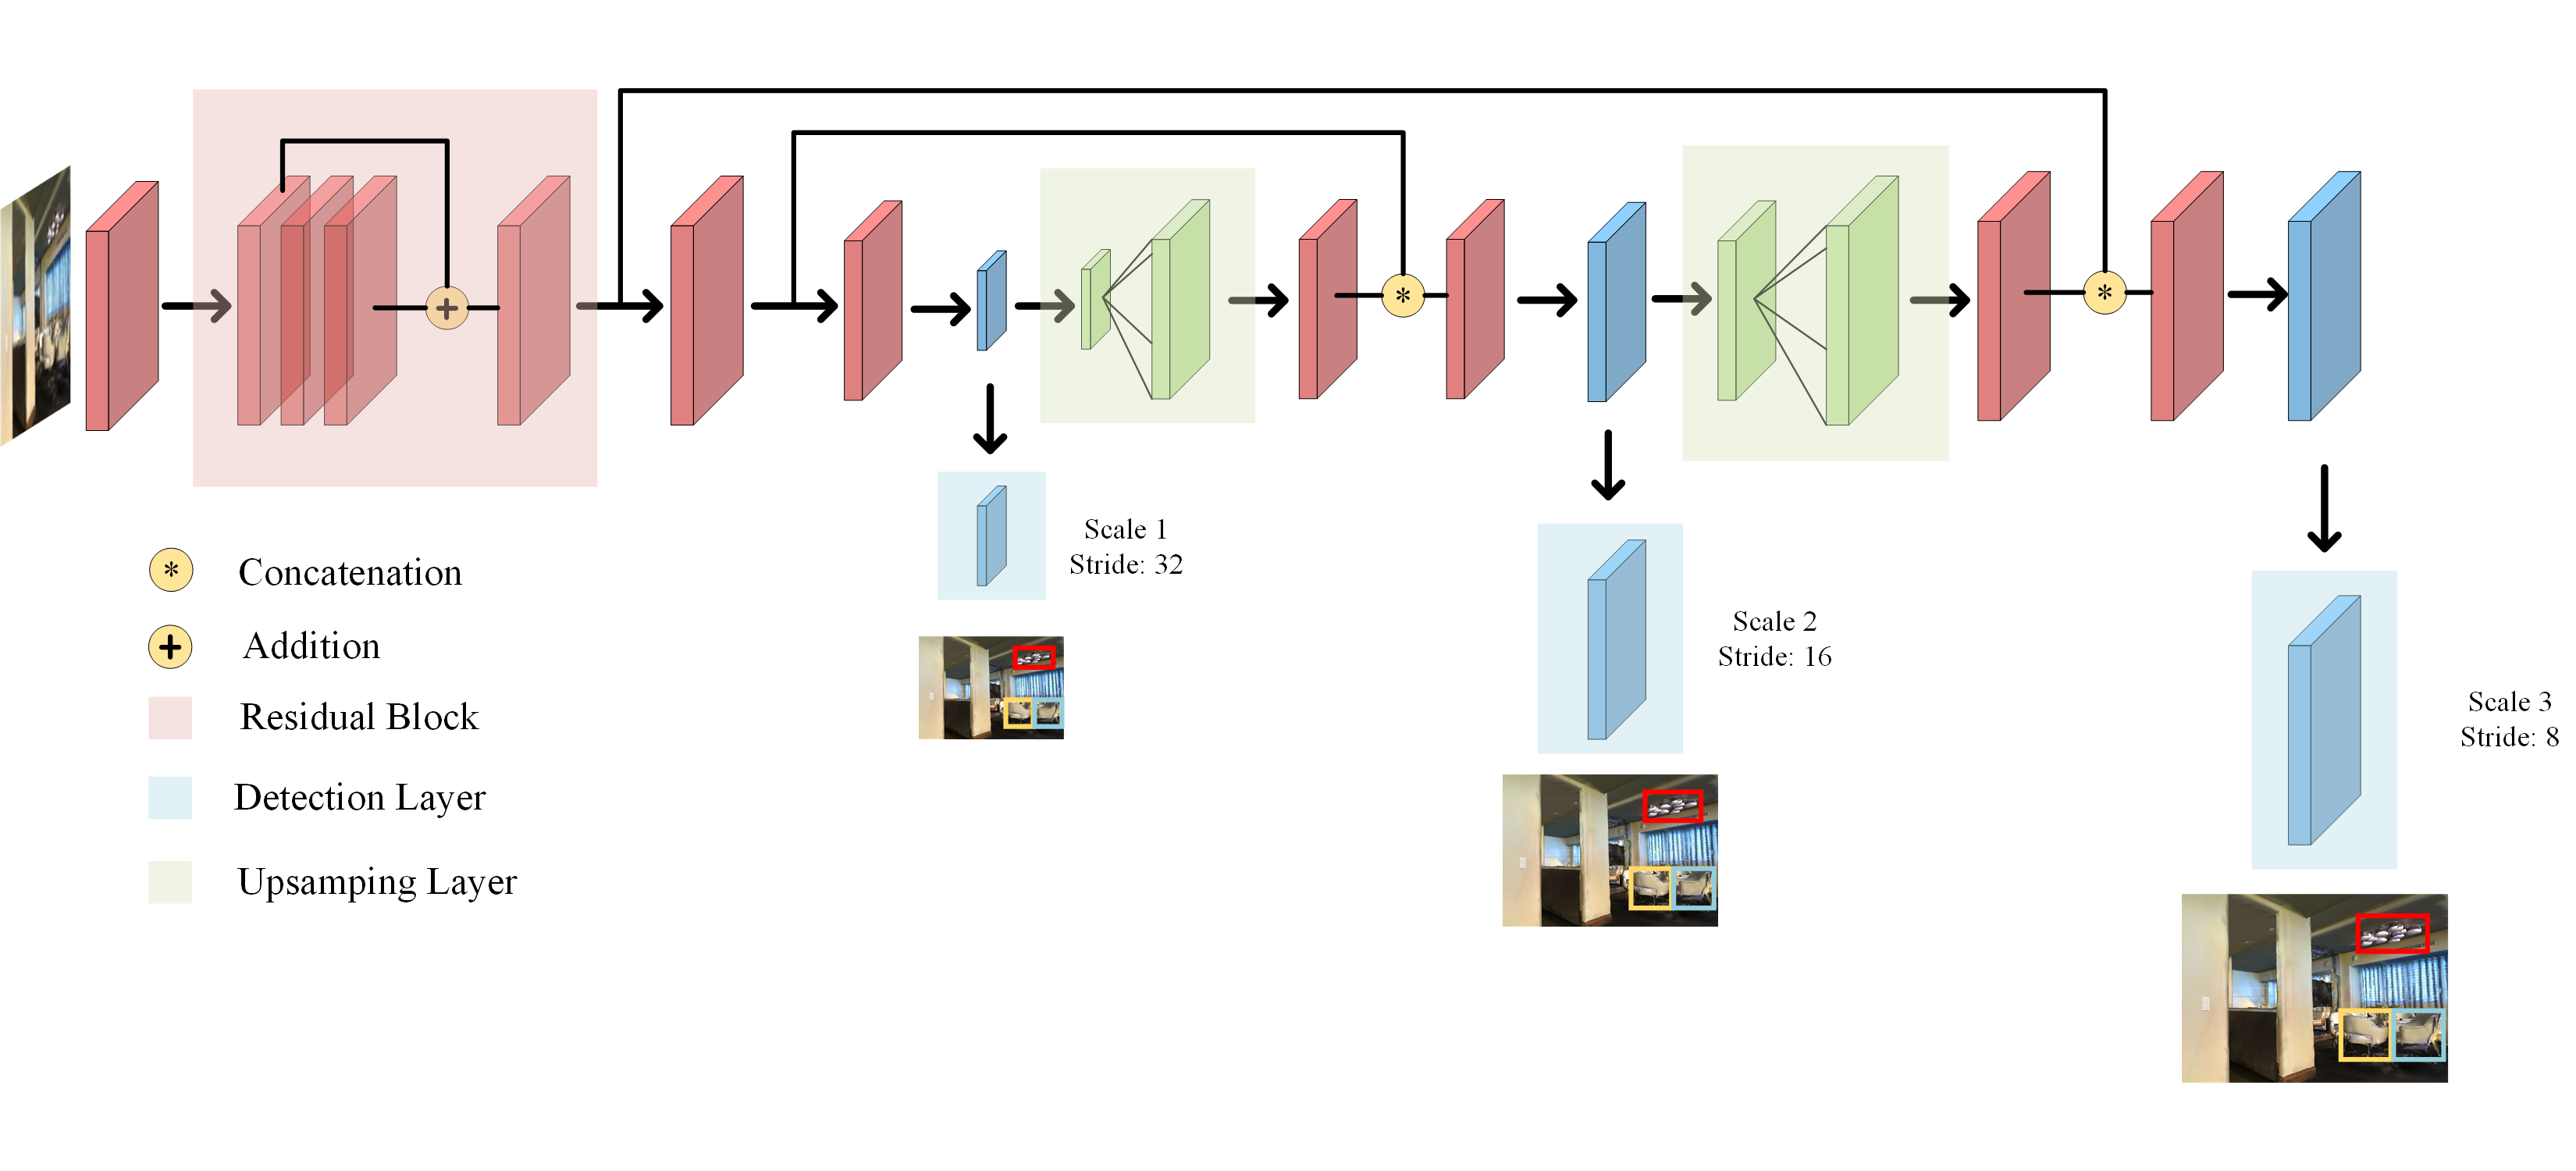
\includegraphics[scale=1]{image04.png}
	\caption{Schema of the proposed architecture for Yolo.}
	\label{image04}
\end{figure*}
\vspace{-1em}
The target detection algorithm has made a great breakthrough. The more popular algorithms can be divided into two categories, one is the R-CNN algorithm based on region proposal (Fast R-CNN and Faster R-CNN). They are two-stage and need to use heuristic methods or CNN network to generate region proposals, and then perform classification and regression on the region proposals \cite{mao2019mini,girshick2015fast}. The other is one-stage algorithms such as Yolo and SSD , which only use a CNN network to directly predict the categories and positions of different targets. The first type of method is more accurate, but slower, but the second type of algorithm is faster, but the accuracy is lower.
	
as the Figure \ref{image04} shows, we use Yolo algorithm, which is detected by a CNN network. It is a single-pipe strategy, and its training and prediction are both end-to-end, so the Yolo algorithm is relatively simple and fast. Then, since Yolo convolves the entire picture, it has a larger field of view in the detection target, and it is not easy to misjudge the background.
\vspace{-1em}
\subsection{Review of Entity Abstraction Component}
	
In order to further consider the degree of matching between the key target information and the instruction information, we introduced entity abstract components to process the characteristic information under the instruction information. We adopt a similar approach to Suhr \cite{suhr2018learning}, replacing phrases in the sentences which refer to previously unseen entities with variables. E.g.,“Walk from kitchen to sofa” turns into “Walk from X1 to Y1”. Here X1 and Y1 are the feature points that match the perceived visual information. We use entity abstract components to extract different types of subjects (streets, restaurants, etc.) and number them in the order of occurrence of sentences \cite{paz2019run}. as the Figure \ref{image05} shows, the number is reset after each instruction is completed, so the model is still a small number of key information is saved, so that the matching efficiency of the overall model is significantly improved \cite{iyer2017learning}. We use an encoder-decoder model with global attention, where the anonymized utterance is encoded using a bidirectional LSTM network.

\begin{equation}
	\centering
	{c}_{i} = \displaystyle\sum_{j=1}^k {\alpha}_{i, j} \cdot s_{j}
\end{equation}

\begin{equation}
	\centering
	{\alpha}_{i, j} = {\frac{exp({h_{i}^{T}Fs_{j}})}{\sum_{j=1}^{k}exp({h_{i}^{T}Fs_{j}})}}
\end{equation}

\begin{equation}
	\centering
	{h}_{i}, {m}_{i} = f({h}_{i-1}, {m}_{i-1}, {c}_{i-1})
\end{equation}

The attention weights ${\alpha}_{i, j}$ are computed using an inner product between the decoder hidden state for the current timestep ${h}_{i}$, and the hidden representation of the source token ${s}_{j}$. Where ${F}$ is a linear transformation. The decoder LSTM cell ${f}$ computes the next hidden state ${h}_{i}$, and cell state ${m}_{i}$ based on the previous hidden and cell states,${h}_{i-1}$,${m}_{i-1}$, the context vector of the previous timestep, ${c}_{i-1}$.

\begin{figure*}[h]
	\centering
	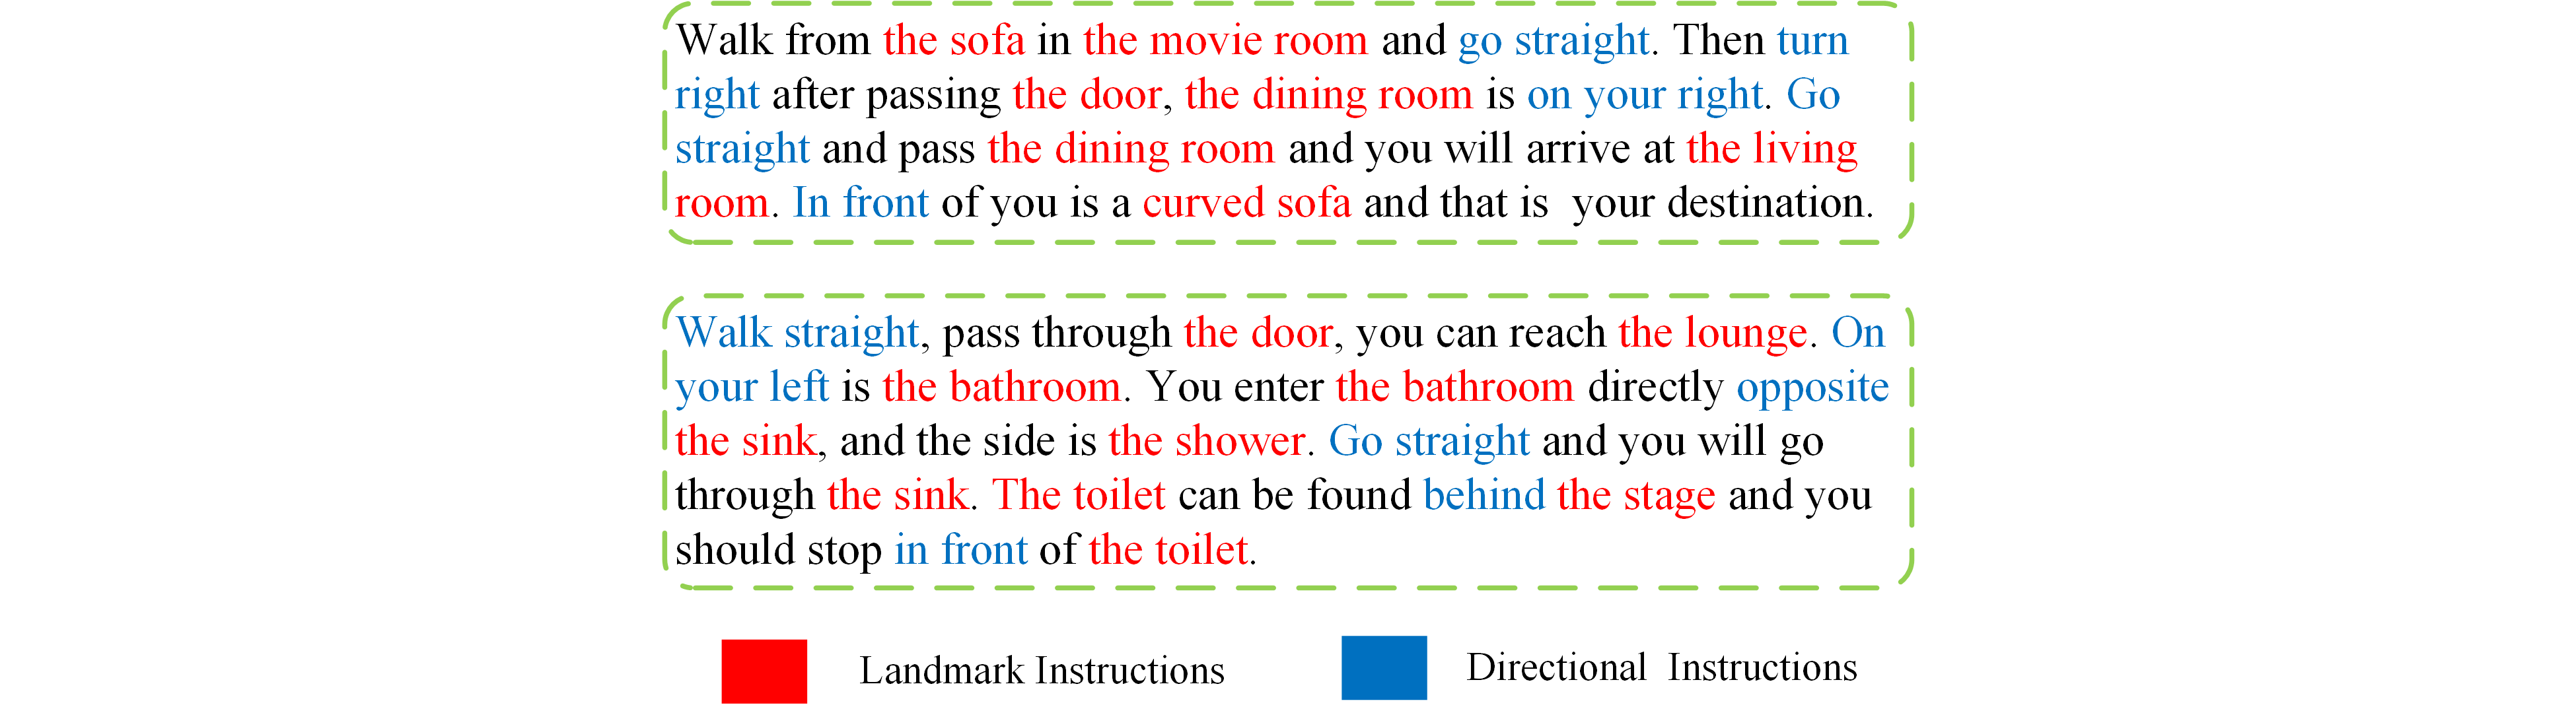
\includegraphics[scale=1]{image05.png}
	\caption{Examples of instruction for navigation. We use entity abstract components to extract different types of subjects (streets, restaurants, etc.) and number them in the order of occurrence of sentences.}
	\label{image05}
\end{figure*}
\vspace{-2em}
\subsection{Vision and Instruction Matching Module}
	
In view of the fact that traditional processing methods only increase the matching effect by increasing the amount, only copy the data set, simply increase the number to improve the accuracy of the matching, or simply complicate the dataset (delete and modify the dataset or add other types of data), these methods still ignore the characteristics of the data set itself. Therefore, our visual instruction matching module is used to determine whether the agent has reached the landmark of the predetermined trajectory, which is the key matching part of the two types of information \cite{vasudevan2021talk2nav}. The image information obtained by the concrete vision is matched with the entity extracted from the language input. In the original visual and language information, the matching of entity information in the data stream is focused on, thereby improving the overall cross-modal matching ability \cite{zhao2021evaluation}.
	
For panoramic images, the orientation features based on the pre-trained Reset-152 and the agent will be input into the visual features of the convolutional neural network (CNN). The institutional embedding dataset for each mode is input as the joint multimodal embedding module so that embedding features can be generated based on intermodal data exchange. Input the perceptual visual features processed by Yolo and the instruction keywords extracted by the entity extraction component to the visual instruction matching module, and set the controller of the scoring module as:

\begin{equation}
	\centering
	{\Psi}_{t}({s}_{t},{h}_{t-1}){\in}{({0},{1})}
\end{equation}

where ${1}$ indicates that the aimed landmark is reached and ${0}$ otherwise. ${{\Psi}_{t}}$ is an Adaptive Computation Time (ACT) LSTM which allows the controller to learn to make decisions at variable time steps. ${h}_{t-1}$ is the hidden state of the controller. In this work, ${{\Psi}_{t}}$ learns to identify the landmarks with the variable number of intermediate navigation steps.

\subsubsection{Track and Instruction Matching Module}

The inspiration for trajectory instruction matching comes from the fact that when people find their way, they will confirm whether they have not deviated from the trajectory when they reach a landmark or need to turn. Some scholars have made bold attempts before. Gordon and others used external memory MT to clearly remember the traversal path of the agent from the newly visited landmark\cite{vasudevan2021talk2nav}. When the agent reaches the iconic location, the memory MT is reinitialized to store the traversed path from the most recently visited landmark. This re-initialization can be understood as focusing on the most recently traversed path in order to better locate and better match the relevant direction indication through the trajectory instruction matching module.

\begin{figure*}[h]
	\centering
	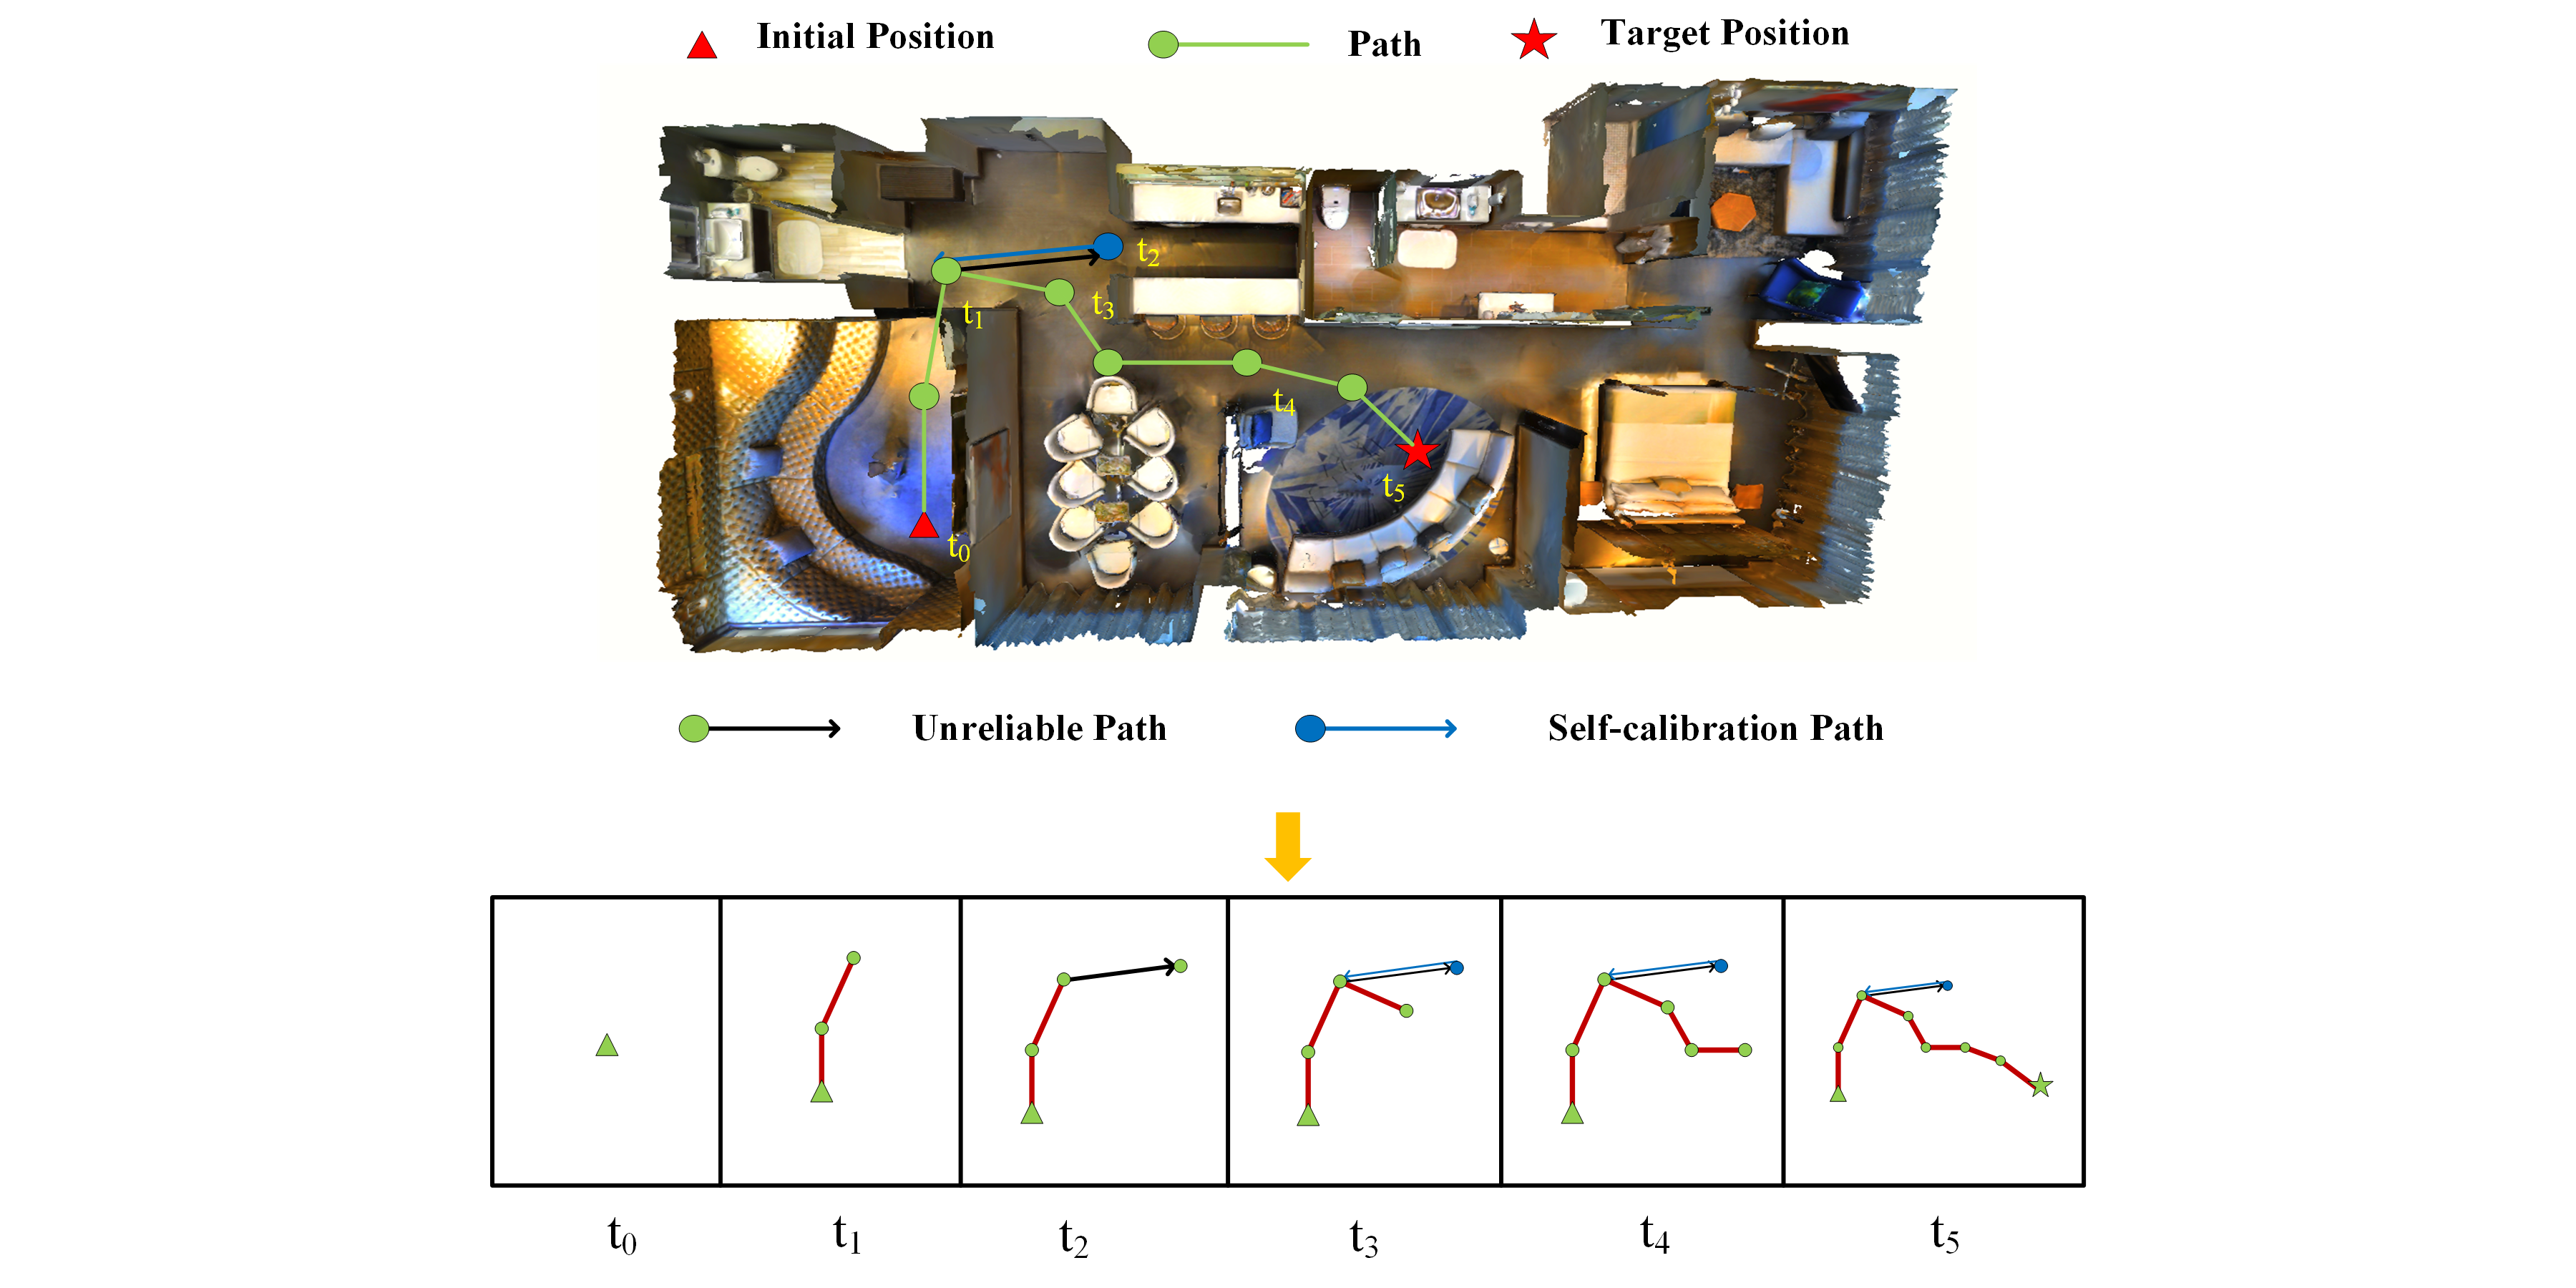
\includegraphics[scale=1]{image06.png}
	\caption{Examples of navigation trajectory. The path is rasterized and written into the memory image.}
	\label{image06}
\end{figure*}

As the Figure \ref{image06} shows, since the agent is in the navigation process, we set up a write module to write the traversed path into the memory and calculate it from the traversal path in the simulation environment. Our writing module tracks the path from the most recently visited key point to the current location. The path is rasterized and written into the memory image. In the image, the path is represented by the red line, the starting point is marked by the blue square. The write module always writes from the center of the memory image to ensure that there is space in all directions. Whenever the coordinates of a new rasterized pixel exceeds the image size, the module incrementally increases the proportion of the stored image until the new pixel is in the image.

By recording the characteristics of the trajectory and inputting the corresponding instructions to the trajectory instruction matching module, the controller of the scoring module is set as:

\begin{equation}
	\centering
	{\varphi}_{t}({m}_{t},{h}_{t-1}){\in}{({0},{1})}
\end{equation}

where ${1}$ indicates that the aimed landmark is reached and ${0}$ otherwise. ${{\varphi}_{t}}$ is an Adaptive Computation Time (ACT) LSTM which allows the controller to learn to make decisions at variable time steps. ${h}_{t-1}$ is the hidden state of the controller. In this work, ${{\varphi}_{t}}$ learns to identify the landmarks with the variable number of intermediate navigation steps.

\subsubsection{Action prediction module}
	
The action at at time ${T}$ is defined as the weighted average of ${{\Psi}_{t}}$ and ${{\varphi}_{t}}$ . For different parts of the trajectory, the input of the action predictor mainly depends on  two inputs ${{\lambda}{\Psi}_{t} + {\varphi}_{t}}$ . For example, when the next key information is not visible, the prediction should rely on ${{\varphi}_{t}}$ ; when the key information is clearly identifiable, both inputs are input to the predictor. After the final data analysis, we determined that when the ${\lambda}$  is equal to 0.75, the overall network effect is the best. The learned matching score will adaptively decide which predictions are trustworthy and how many are passed in each step. This adaptive fusion can be understood as a calibration system of two complementary subsystems for motion prediction. The calibration method needs time or situation dependent. In this case, the input of the action predictor is enriched to the greatest extent, more accurate navigation actions are trained, and then the navigation trajectory with less error is serialized.
	
\subsection{Learning Detail}
	
The model is trained in a supervised manner. We follow the student-forcing approach to train our models. In each step, the monitoring signal with motion in the direction of the next landmark trains the motion prediction module. We use cross-entropy loss to train the action module and the matching module because they are planned as classification tasks. The total loss is the sum of the losses of all modules:
	
\begin{equation}
	\centering
	{Loss}_{all} = {Loss}_{vision-matching} + {Loss}_{track-matching} + {Loss}_{action}
\end{equation}

The loss of the two matching modules only takes effect at the landmarks of the landmarks, and these landmarks are more than the road nodes for calculating the motion loss and trajectory error loss. Therefore, we first train the matching networks separately for the matching task, and then integrate them with other components into overall training. We use ${Loss}_{all}$ to train the entire network.

\section{Experiments}
	
\subsection{Experimental Settings}
	
\textbf{Dataset.} We use the Room-to-Room (R2R) vision-and-language navigation dataset for our experimental evaluation\cite{anderson2018vision}. In this task, the agent starts at a certain location in an environment and is provided with a human-generated navigation instruction, that describes a path to a goal location. The agent needs to follow the instruction by taking multiple discrete actions (e.g. turning, moving) to navigate to the goal location, and executing a “stop” action to end the episode. Note that differently from some robotic navigation settings, here the agent is not provided with a goal image, but must identify from the textual description and environment whether it has reached the goal.
	- the Matterport3D navigation graphs, where each path consists of 5 to 7 discrete viewpoints and the average physical path length is 10m. Each path has three instructions written by humans, giving 21.5k instructions in total, with an average of 29 words per instruction. The dataset is split into training, validation, and test sets. The validation set is split into two parts: seen, where routes are sampled from environments seen during training, and unseen with environments that are not seen during training. All the test set routes belong to new environments unseen in the training and validation sets.

\textbf{Evaluation metrics.} Following previous work on the R2R task, our primary evaluation metrics are navigation error (NE), measuring the average distance between the end-location predicted by the follower agent and the true route’s end-location, and success rate (SR), the percentage of predicted end-locations within 3m of the true location. As in previous work, we also report the oracle success rate (OSR), measuring success rate at the closest point to the goal that the follower has visited along the route, allowing the agent to overshoot the goal without being penalized.

\textbf{Implementation details.} We produce visual feature vectors v using the output from the final convolutional layer of a ResNet trained on the ImageNet classification dataset. These visual features are fixed, and the ResNet is not updated during training. To better generalize to novel words in the vocabulary, we also experiment with using BERT to initialize the word-embedding vectors. We generate dynamic filters with 512 channels using a linear layer with dropout (p = 0.5).In our attention module, q and K have 128 channels and we apply a ReLU non-linearity after the linear transformation. For our action selection, we apply dropout with p = 0.5 to the policy hidden state before feeding it to the linear layer.
\vspace{-2em}
\subsection{Ablation Study}
\vspace{-2em}
\begin{table*}[h]
	\centering
	\caption{The ablation study of our architecture on the R2R validation group and our baseline model is the Speaker-Follower model. When the key information matching module and the trajectory self-correction module are added, the effect of the whole model is better.}
	{\begin{tabular}[c]{ccccccccccccc}
			\toprule[1pt]
			\multirow{2}{*}{{\textbf{Model}}} & \multicolumn{4}{c}{{\textbf{Validation Seen}}} & \multicolumn{4}{c}{{\textbf{Validation Unseen}}}\\
			
			& \textbf{SR}$\uparrow$ & \textbf{NE}$\downarrow$ & \textbf{OSR}$\uparrow$ & \textbf{SPL}$\uparrow$	& \textbf{SR}$\uparrow$ & \textbf{NE}$\downarrow$ & \textbf{OSR}$\uparrow$ & \textbf{SPL}$\uparrow$ & \\
			\toprule[1pt]
			
			Baseline   & 0.63 & 3.4 & 0.71 & - & 0.38 & 6.68 & 0.42 & -\\
			Cross-model guide  & 0.68 &  3.31 &  0.76 & 0.59 & 0.41 & 5.94 & 0.53  & 0.35 \\
			Self-calibration    & 0.64 & \textbf{3.20} & 0.76 & 0.52 & 0.42 & \textbf{5.57} & 0.45 & 0.34 \\
			KIM-Net & \textbf{0.69} &  3.23 & \textbf{0.78} & \textbf{0.64} & \textbf{0.46} & 5.63 & \textbf{0.57} & \textbf{0.39} \\
			
			\bottomrule[1pt]
		\end{tabular}
		\label{table_1}}
\end{table*}
\vspace{-2em}
\begin{table*}[h]
	\centering
	{\begin{tabular}[c]{cccccccccc}
			\toprule[1pt]
			\multirow{2}{*}{{\textbf{Method}}} & \multirow{2}{*}{{\textbf{Num}}} & \multicolumn{1}{c}{{\textbf{Cross-model}}}  & \multicolumn{1}{c}{{\textbf{Track}} } &\multicolumn{4}{c}{{\textbf{Test Seen}}} \\
			
			& &\textbf{Guide} &\textbf{Self-calibration} & \textbf{SR}$\uparrow$ & \textbf{NE}$\downarrow$ & \textbf{OSR}$\uparrow$ & \textbf{SPL}$\uparrow$\\
			\toprule[1pt]
			
			Speaker-Follower   & & & & 0.36 & 6.69 & 0.42 & 0.28 \\
			\toprule[1pt]
			\multirow{3}{*}{KIM-Net}  &1& $\surd$ & & 0.43 &  5.97 &  0.51 & 0.34  \\
			   &2& & $\surd$ & 0.41 & \textbf{5.59} & 0.43 & 0.33  \\
				 &3& $\surd$ & $\surd$ & \textbf{0.47} &  5.76 & \textbf{0.53} & \textbf{0.39} \\
			\bottomrule[1pt]
		\end{tabular}
		\label{table_2}}
\end{table*}
The results presented in Table \ref{table_1} show, we test the impact of our implementation choices on VLN in our ablation study. First, we compare the KIM-Net model with a model that uses a simple replication data set to expand the data set to discuss the impact of the key information matching module on the entire network. Then, we introduced the importance of using the trajectory self-correction module to correct the entire navigation task.

\textbf{Cross-model guide module.}As the results show, the performance of the key information matching model in data set processing largely exceeds the traditional data enhancement method of VLN. This is because the model can more accurately dig out the inner connection between the perceptual vision and text instructions under the input data set. Compared with the baseline model using purely replicated data sets, our Cross-model guide module improves the success rate by 5.

\textbf{Track self-calibration module.}Our method is significantly better than the self-monitoring agent using greedy decoding. When the progress marker can use the features of each navigable direction previously accessed, but the trajectory self-correction module is not available, the performance will not increase significantly (36 SR) . However, the use of the gated attention mechanism is good for extracting the overlap between the position of the landmark under the text instruction and the real trajectory, which means that the network can use this information to improve action selection. Compared with the baseline model that uses pure soft attention to compare the error of the entire trajectory, our method can achieve a moderate gain (41 SR), which reflects the purpose of intelligent navigation.

\begin{figure}[h]
	\centering
	\subfigure[Validation Seen]{
		\begin{minipage}[t]{0.33\linewidth}
			\centering
			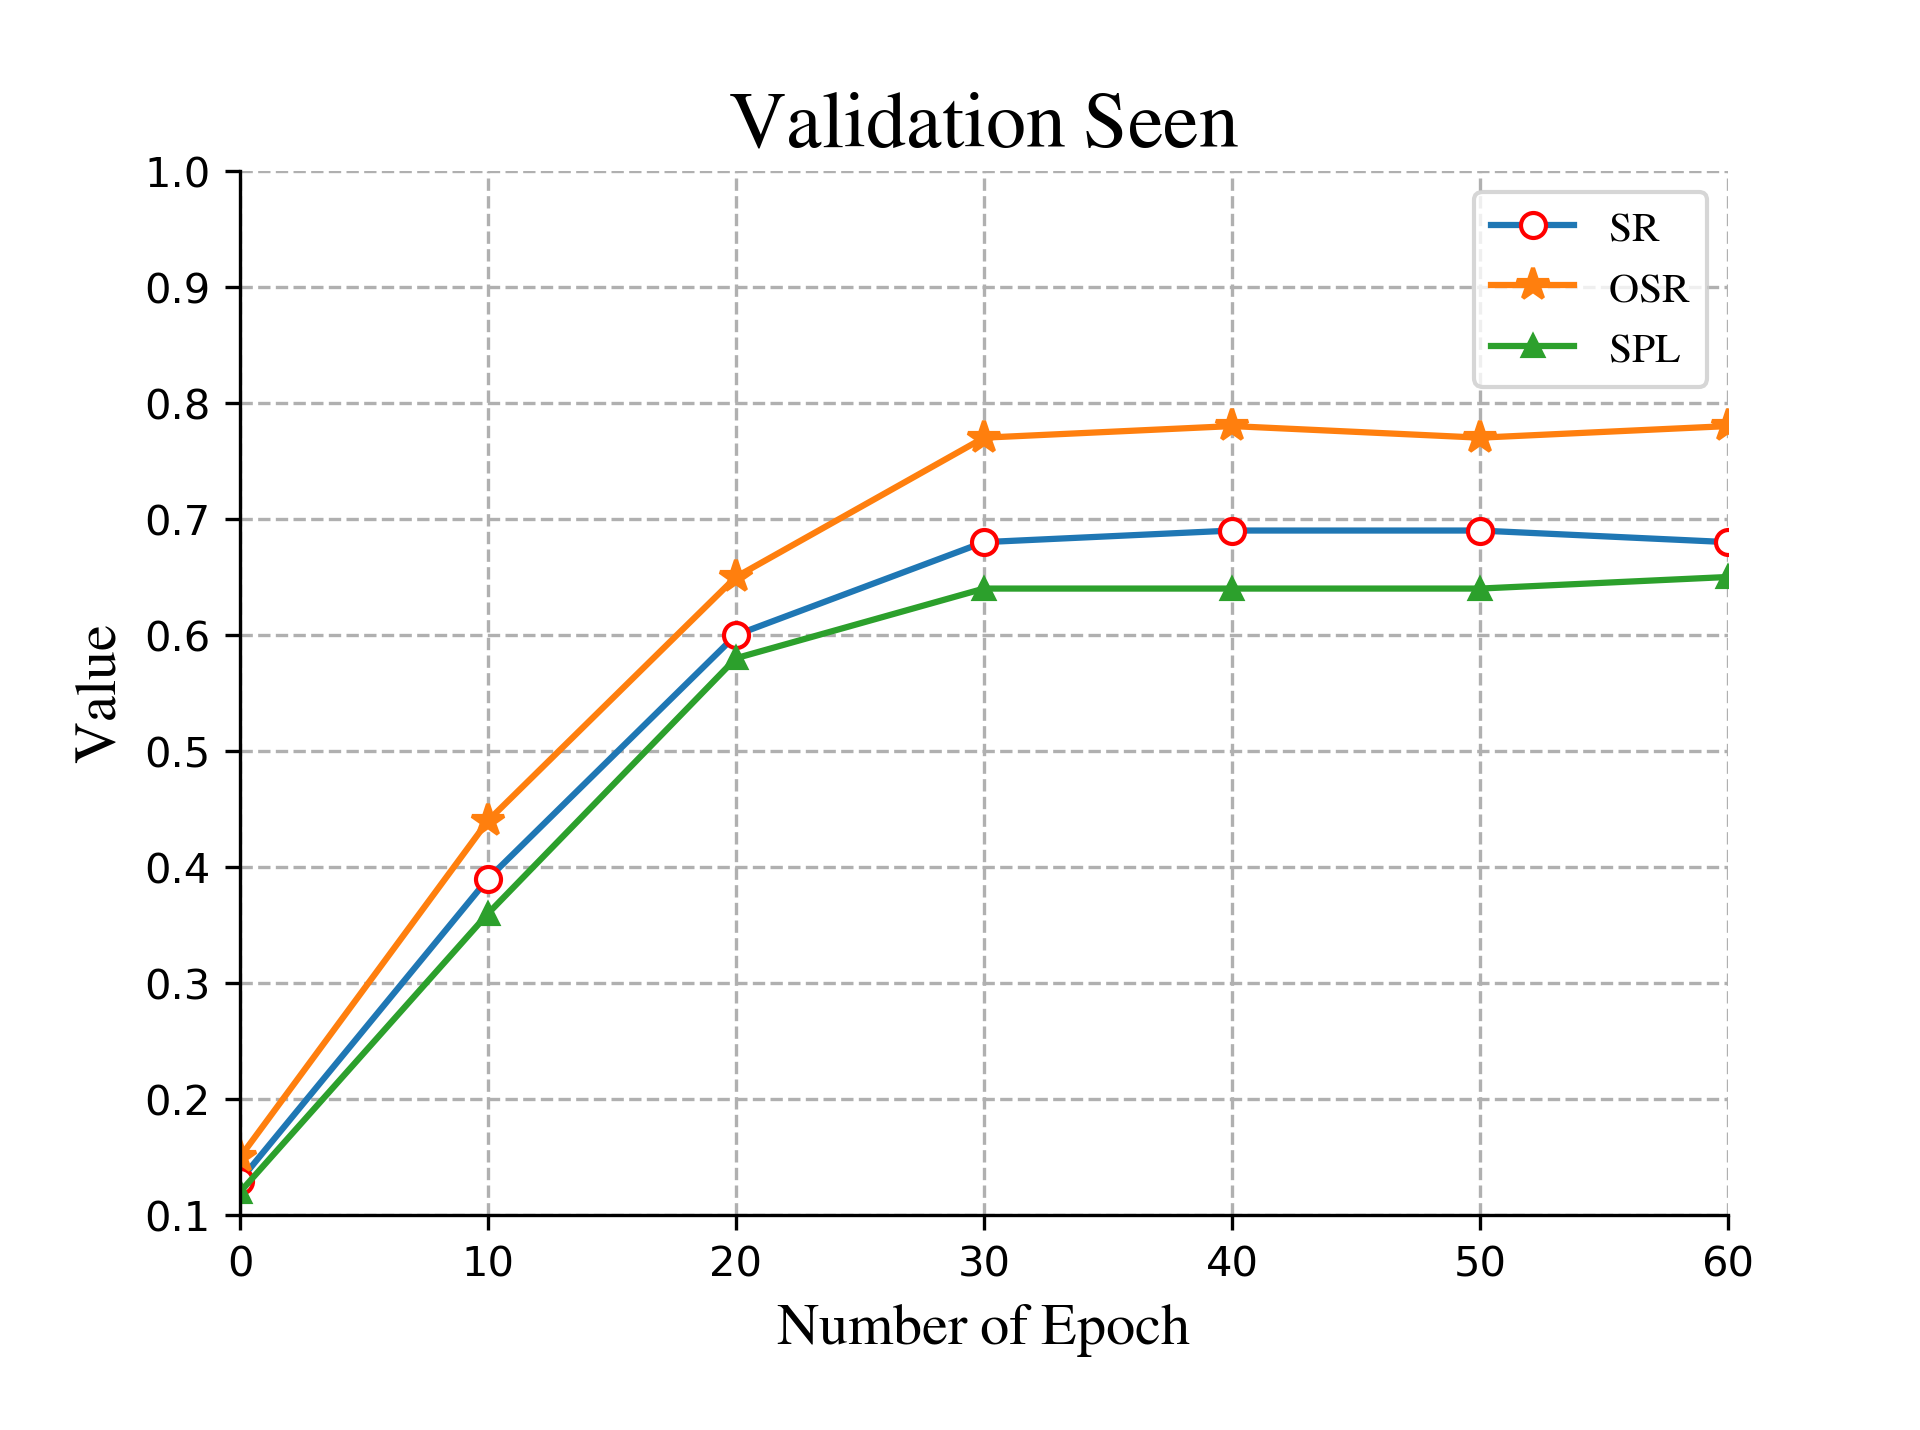
\includegraphics[width=2in]{Figure_1.png}
		\end{minipage}%
	}%
	\subfigure[Validation Unseen]{
		\begin{minipage}[t]{0.33\linewidth}
			\centering
			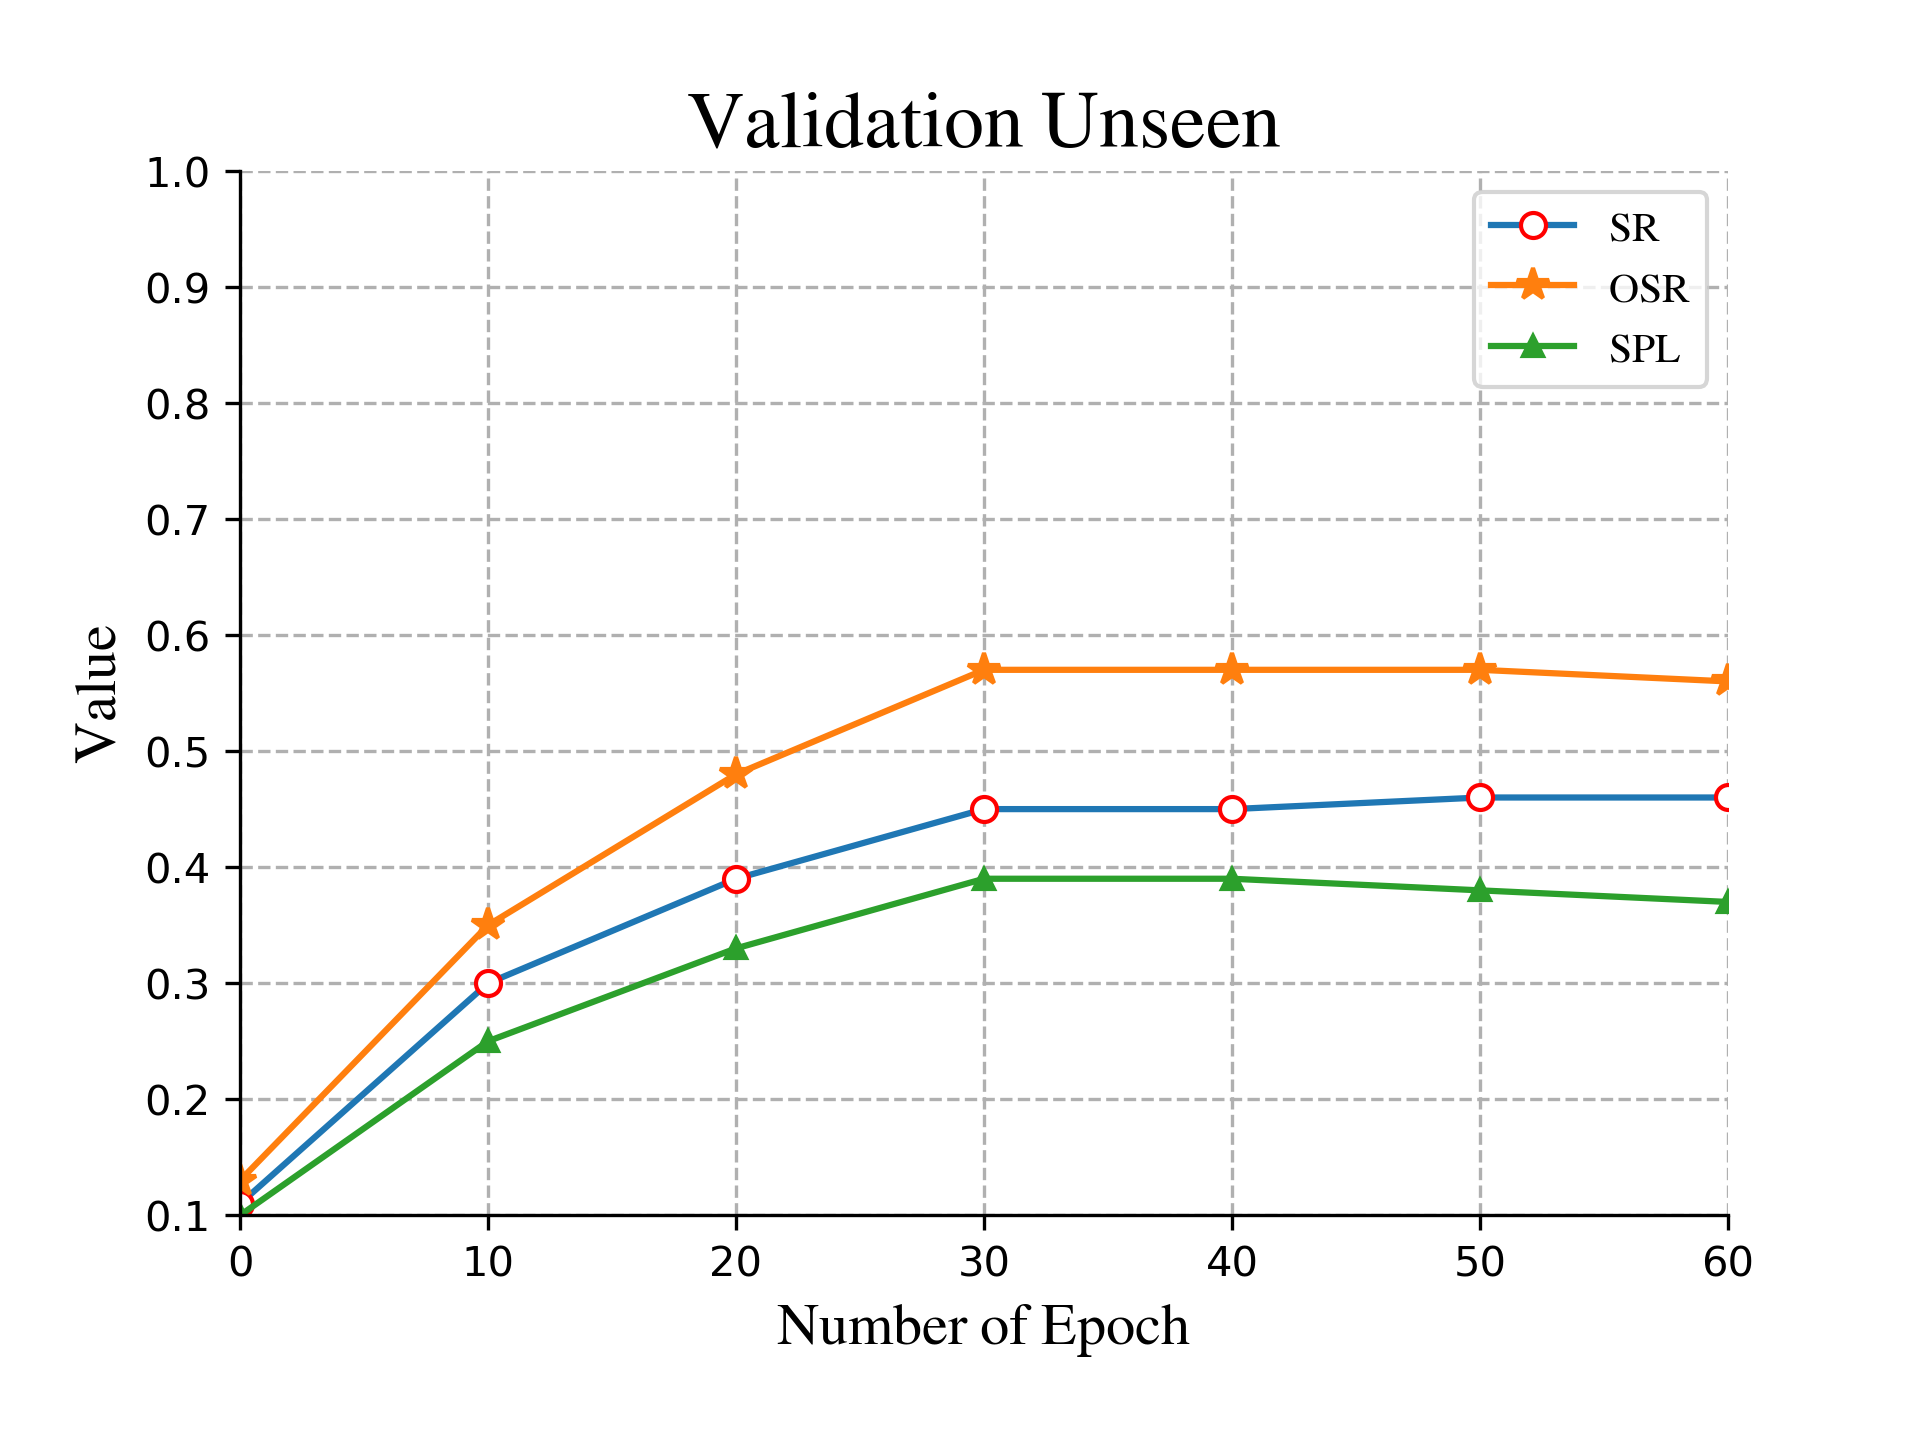
\includegraphics[width=2in]{Figure_2.png}
		\end{minipage}%
	}%
	\subfigure[Test Unseen]{
		\begin{minipage}[t]{0.33\linewidth}
			\centering
			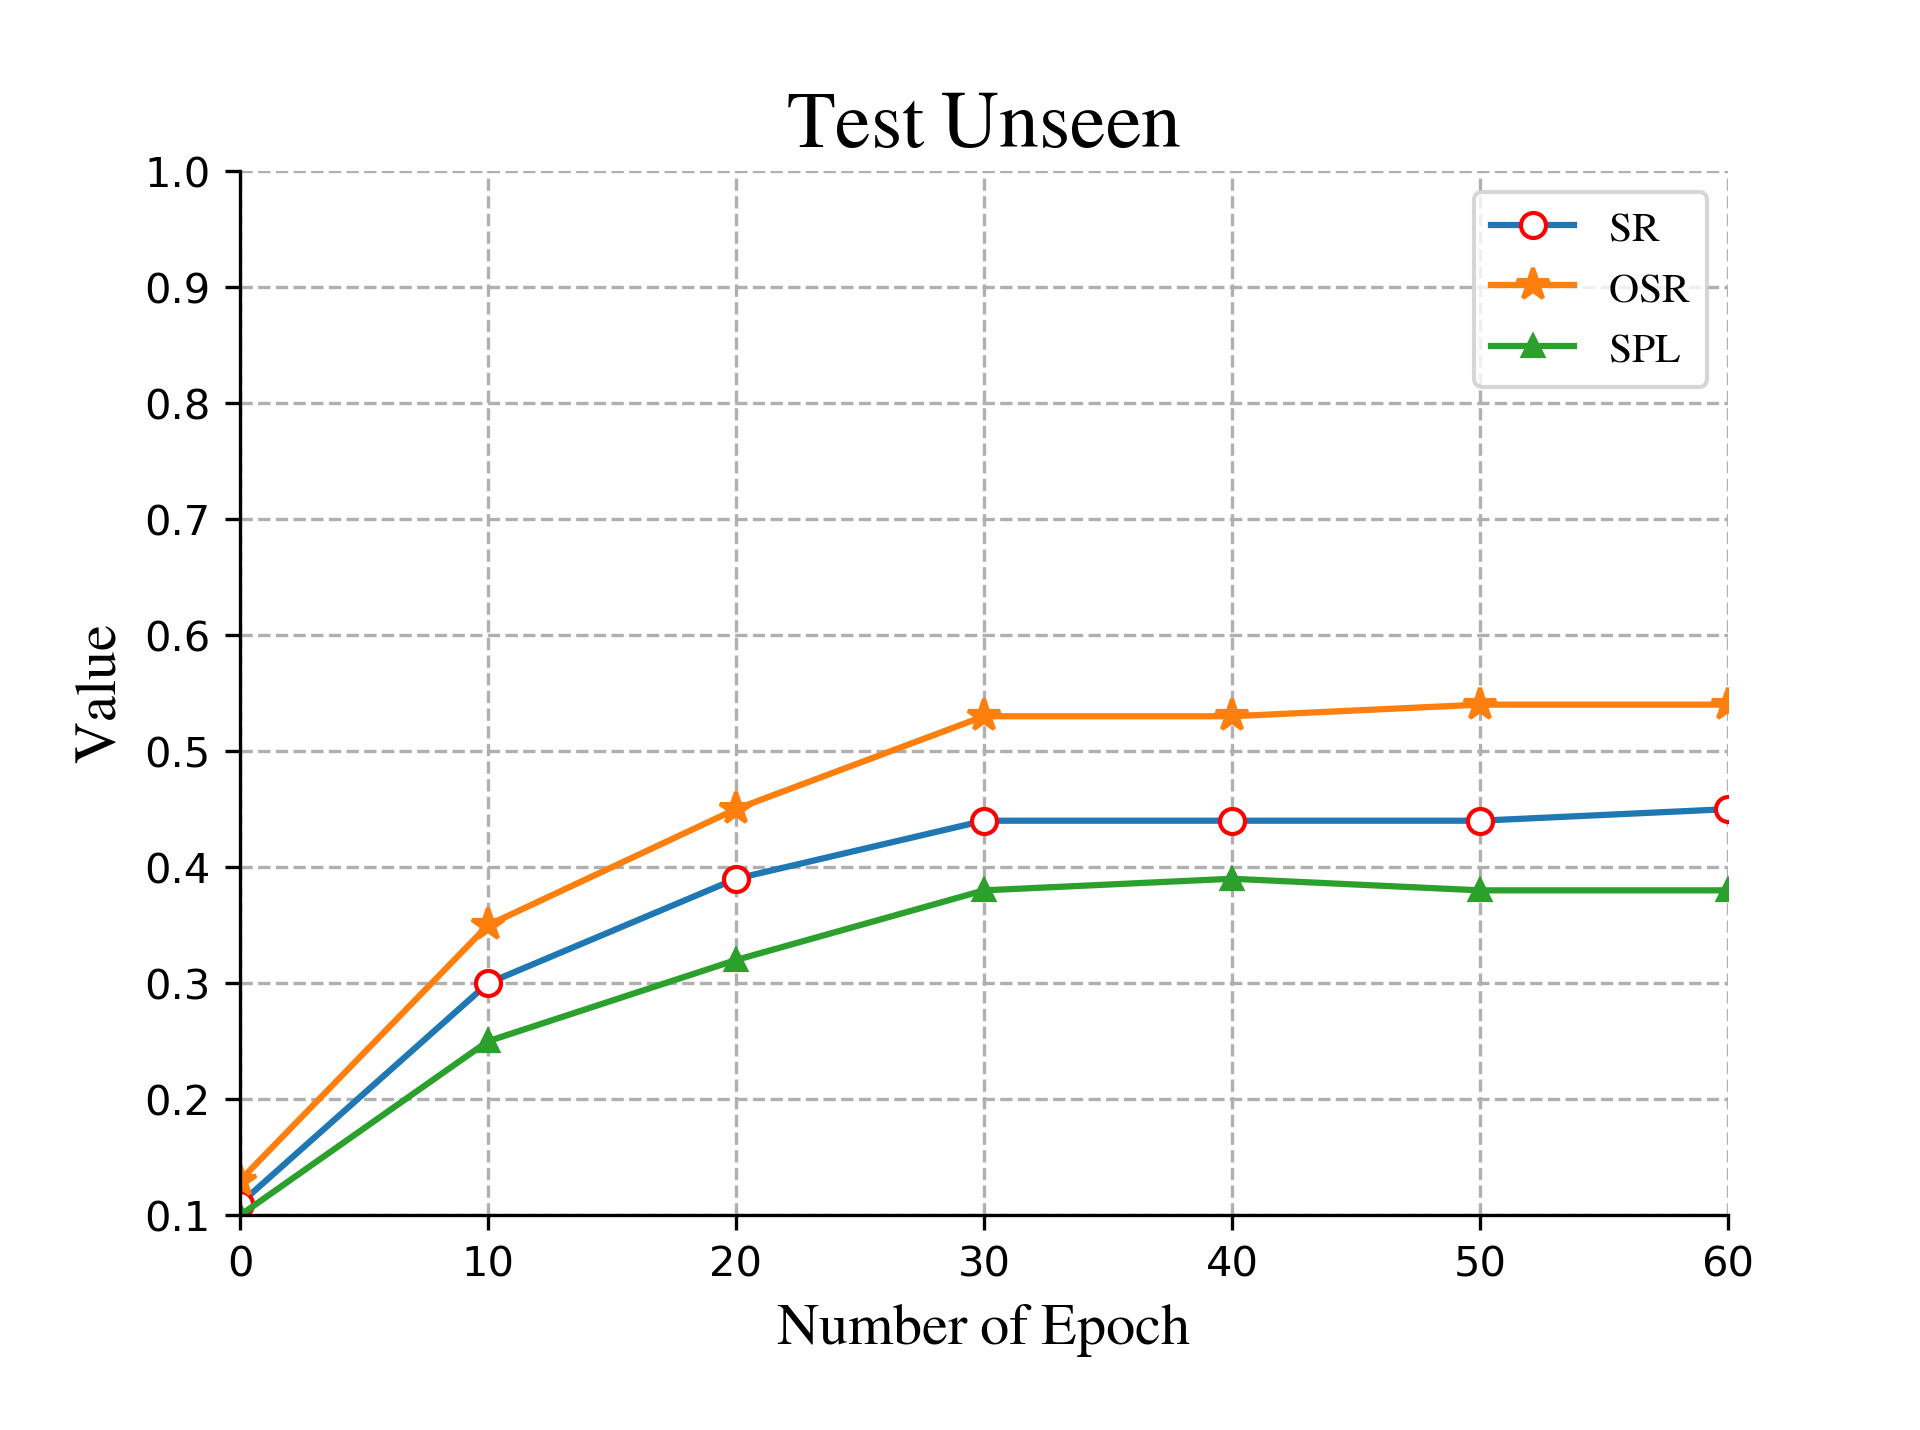
\includegraphics[width=2in]{Figure_3.png}
		\end{minipage}%
	}%
	\centering
	\caption{ Comparison of performance on the different condition: (a) Validation Seen, (b) Validation Unseen, and (c) Test Unseen.}
\end{figure}

\begin{figure}[h]
	\begin{minipage}{0.5\textwidth}
		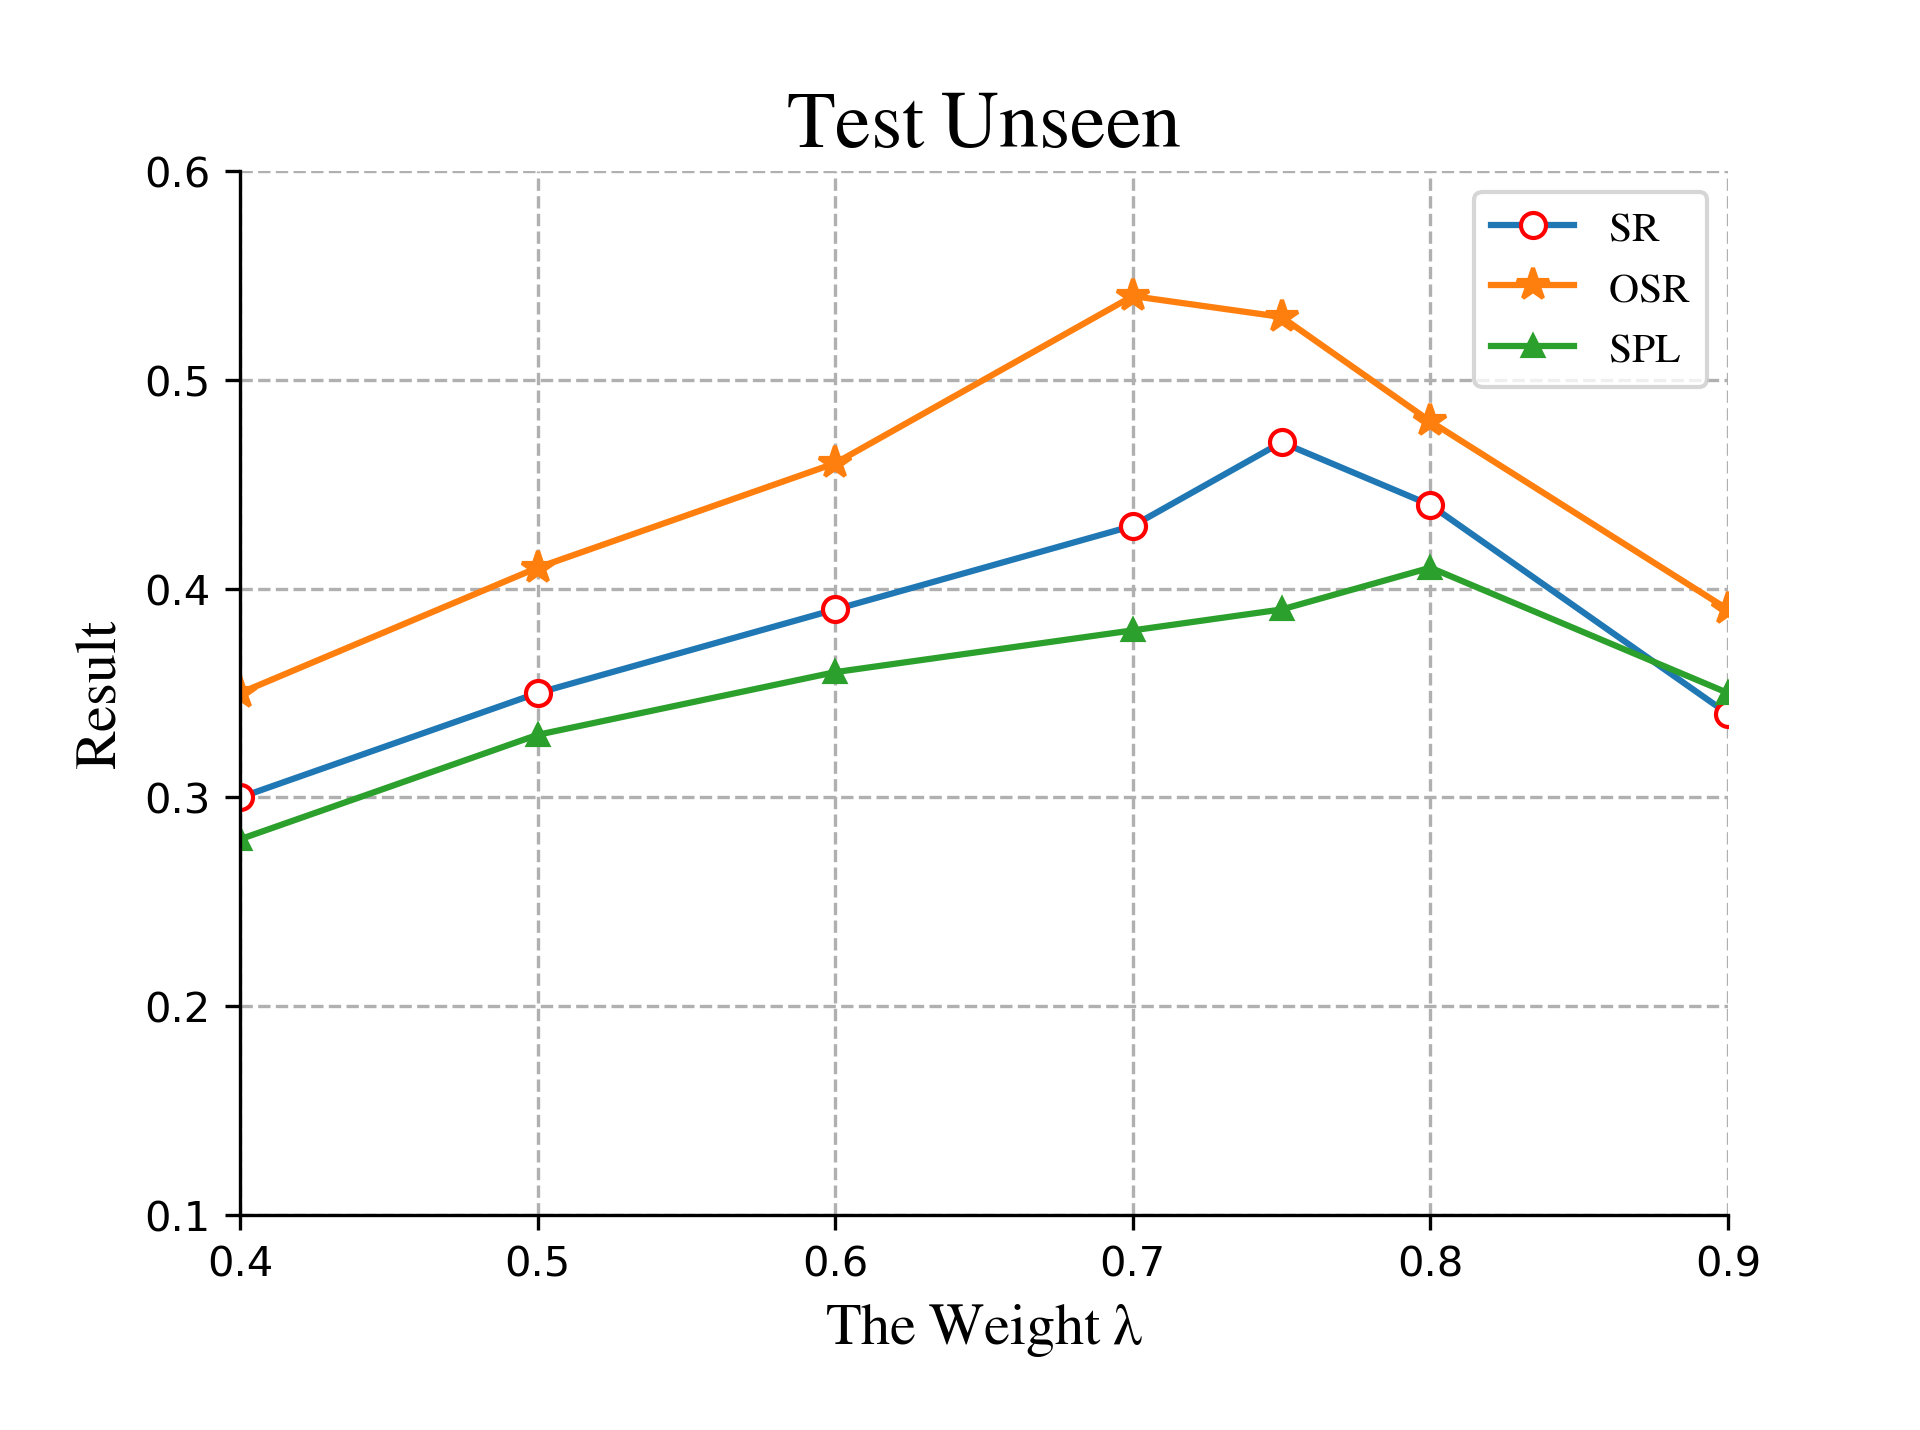
\includegraphics[width=2.5in]{Figure_4.png}
	\end{minipage}
	\hfill
	\begin{minipage}{0.5\textwidth}
		\begin{table}[H]
			\vspace{-2em}
			\centering
			\caption{Comparison of the Test Unseen Set.}
			{\begin{tabular}[c]{ccccccccccccc}
					\toprule[1pt]
					\multirow{2}{*}{{\textbf{The Weight ${\lambda}$}}} & \multicolumn{4}{c}{{\textbf{Test Unseen}}} \\
					
					& \textbf{SR}$\uparrow$ & \textbf{OSR}$\uparrow$ & \textbf{SPL}$\uparrow$	&  \\
					\toprule[1pt]
					
					0.4   & 0.30 & 0.35 & 0.28 \\
					0.5  & 0.35 &  0.41 & 0.33  \\
					0.6    & 0.39 & 0.46 & 0.36  \\
					0.7 	& 0.43 & \textbf{0.54} & 0.38 \\
					0.75   & \textbf{0.47} &  0.53 & 0.39 \\
					0.8   & 0.44 & 0.48 & \textbf{0.41} \\
					0.9   & 0.34 & 0.39 & 0.35 \\
					\bottomrule[1pt]
				\end{tabular}
				\label{table_3}}
		\end{table}
	\end{minipage}
	\caption{Comparison of performance on the different weight of Scoring module. The best result is approximately obtained when the  is equal to 0.75.}
\end{figure}
We compared different results and plotted images to further observe the changes in the results of different training epoch. when ${{\lambda}}$ was equal to 0.75 in the formula ${{\lambda}{\Psi}_{t} + {\varphi}_{t}}$ in the KIM-net model, the effect of the entire model was optimal.

\section{Related Work}
In order to improve the accuracy of visual language navigation tasks, many scholars \cite{fried2018speaker,hwang2021joint,majumdar2020improving,ma2019regretful,wang2019reinforced,zhu2020vision} have made lots of contributions. The Speaker-Follower model is proposed in Fried. The model is mainly divided into two modules: Speaker module and Follower module. Speaker outputs the corresponding language label according to the path, and Follower is responsible for outputting the path according to the input text command, so that by duplicating the original data set The function of expanding the data set is achieved, and the action space of the environment has been changed. The original one can only rotate 90 degrees stiffly to any angle, which increases the freedom of the action space and makes it more accurate decision; Zhu made an integration of all the previous methods, first combining the three-alignment mechanism of seq2seq, reinforcement- learning and imitation learning, and adding the structure of the graph built in the entire scene, and optimizing the specific loss function to adapt to the new algorithm framework. However, the model proposed by the author still ignores the key information of the entire navigation task, that is, typical landmark objects or obvious location words, and the error between the real trajectory and the text instruction, which leads to the effect of the entire model is still not ideal. Therefore, this paper proposes the KIM-Net model. In the network, we propose two main modules, the visual instruction matching module and the trajectory instruction matching module. The detailed information under the navigation task is deeply excavated, and this method fundamentally solves the above-mentioned problems.

\section{Conclusion}
Conventional navigation focuses on pre-constructing a map of the entire scene, and marking the initial location and destination location. The most suitable trajectory is derived by beam search or greedy algorithms, but the visual language navigation based on deep learning focuses on vision and text The navigation behavior is deduced, in which the visual and text processing are relatively independent, and each is processed by the more mature algorithms in the field, and then simply aligned and spliced, and the appropriate navigation behavior is judged under supervision. This kind of work undoubtedly saves labor costs and time costs, making it more generalizable. This research proposes a new type of deep neural network model KIM-Net as an effective tool to solve VLN tasks. The proposed model aims to use the past temporal context and the multi-modal background extracted with the joint multi-modal embedding module. In addition, KIM-Net, a new greedy local search algorithm with backtracking function, improves the task success rate and search efficiency. Finally, we verify the advantages of the proposed model through various experiments using the R2R benchmark dataset.
	
	%\begin{acknowledgements}
	
	%This research was funded by the National Natural Science Foundation of China under Grants 61872073, 61973093, 61901098, 61971118 and 61973063; the National Key Robot Project grant number$\backslash$2017YFB1300900; Shenyang NEU New Industrial Technology Research Institute (17-500-8-01). 
	
	%\end{acknowledgements}
	
\section*{Declarations}
\subsection*{Funding}
	
	%This research was funded by the National Natural Science Foundation of China under Grants 61872073, 61973093, 61901098, 61971118 and 61973063; the National Key Robot Project grant number$\backslash$2017YFB1300900; Shenyang NEU New Industrial Technology Research Institute (17-500-8-01). 
	
\subsection*{Conflicts of Interest/Competing Interests}
	
The authors declare that they have no conflicts of interest, and they have no competing financial interests or personal relationships that could have appeared to influence the work reported in this paper.
	
\subsection*{Availability of Data and Material}
	
All data generated or analysed during this study are included in this published article and its supplementary information files.
	
\subsection*{Code Availability}
	
Not applicable.
	
\subsection*{Authors' Contributions}
	
	%\textbf{Zixi Jia:} Methodology, Software, Writing - review and editing. \textbf{Lele Xue:} Conceptualization, Methodology, Investigation, Writing - original draft. \textbf{Jingyu Ru:} Validation, Formal analysis, Visualization, Software. \textbf{Zhou Wang:} Validation, Conceptualization, Visualization. \textbf{Minglin Dong:} Validation, Visualization, Editing. \textbf{Sikai Yang:} Software, Review, Editing. \textbf{Jiao Li:} Validation, Wring - review, Editing.
	
\subsection*{Ethics Approval}
	
Not applicable.
	
\subsection*{Consent to Participate}
	
Not applicable.
	
\subsection*{Consent for Publication}
	
Not applicable.
	
	% Authors must disclose all relationships or interests that 
	% could have direct or potential influence or impart bias on 
	% the work: 
	%
	% \section*{Conflict of interest}
	%
	% The authors declare that they have no conflict of interest.
	
	
	% BibTeX users please use one of
	%\bibliographystyle{spbasic}      % basic style, author-year citations
	%\bibliographystyle{spmpsci}      % mathematics and physical sciences
	%\bibliographystyle{spphys}       % APS-like style for physics
	%\bibliography{}   % name your BibTeX data base
	
	% Non-BibTeX users please use
	%\begin{thebibliography}
	%
	% and use \bibitem to create references. Consult the Instructions
	% for authors for reference list style.
	%
	%\reftitle{References}
	\bibliographystyle{ieeetr}
	\bibliography{coling}
	
	%\noindent \textbf{Zixi Jia} received the Ph.D. degree in pattern recognition and intelligent systems from Northeastern University, Shenyang, China, in 2009, where he is currently an Associate Professor and the Vice Dean of Faculty of Robot Science and Engineering. His research interests include artificial intelligence, robotics, big data and wireless sensor networks.\par
	
	%\noindent \textbf{Lele Xue} a graduate student of Faculty of Robot Science and Engineering, Northeastern University,Shenyang,China. His research intersts include computer vision and pattern recognition.\par
	
	%\noindent \textbf{Jingyu Ru}  received the  Ph.D. degrees in Northeastern University, Shenyang, China, in 2019. He is currently a post doctor as a staff in Robot Science and Engineering in Northeastern University, China. His research interests include artificial intelligence, big data, wireless sensor networks and robotics.\par
	
	%\noindent \textbf{Zhou Wang} a graduate student of Faculty of Robot Science and Engineering, Northeastern University,Shenyang,China. His research interst is computer vision.\par
	
	%\noindent \textbf{Minglin Dong} a graduate student of Faculty of Robot Science and Engineering, Northeastern University,Shenyang,China.The research intersts  include computer vision, natural language processing and multimodal fusion\par
	
	%\noindent \textbf{Sikai Yang} a graduate student of Faculty of Robot Science and Engineering, Northeastern University,Shenyang,China.The research interst is computer vision. \par
	
	%\noindent \textbf{Jiao Li} a graduate student of Faculty of Robot Science and Engineering, Northeastern University,Shenyang,China.The research interst  is  natural language processing. \par
	
	
	
\end{document}
% end of file template.tex

